\chapter{Projeto} \label{sec:project}

Nesta seção, apresenta-se a metodologia proposta para a investigação das perguntas de pesquisa estabelecidas no presente estudo, buscando-se analisar, através da aplicação do arcabouço teórico das áreas de Teoria dos Grafos, Redes Complexas e Análise de Redes Sociais, o impacto do círculo social de estudantes do ensino superior sobre seu desempenho acadêmico. Para tanto, o projeto divide-se em três etapas: (i) coleta de dados, compreendendo a elaboração e aplicação do instrumento de pesquisa, assim como a coleta de informações referentes às notas da população pesquisada e a anonimização dos dados; (ii) reconstrução e associação, que aborda a transformação dos dados coletados em redes complexas e a reconciliação das duas fontes de dados; e (iii) análise, que busca extrair inferências a partir dos dados combinados e responder concretamente às perguntas de pesquisa levantadas.

Na Figura \ref{fig:process}, apresenta-se uma visão geral sobre a metodologia proposta, incluindo as três etapas enumeradas. Atenção especial é dada aos processos que lidam com dados sensíveis (expressos em vermelho).

\begin{figure}[ht]
    \centering
    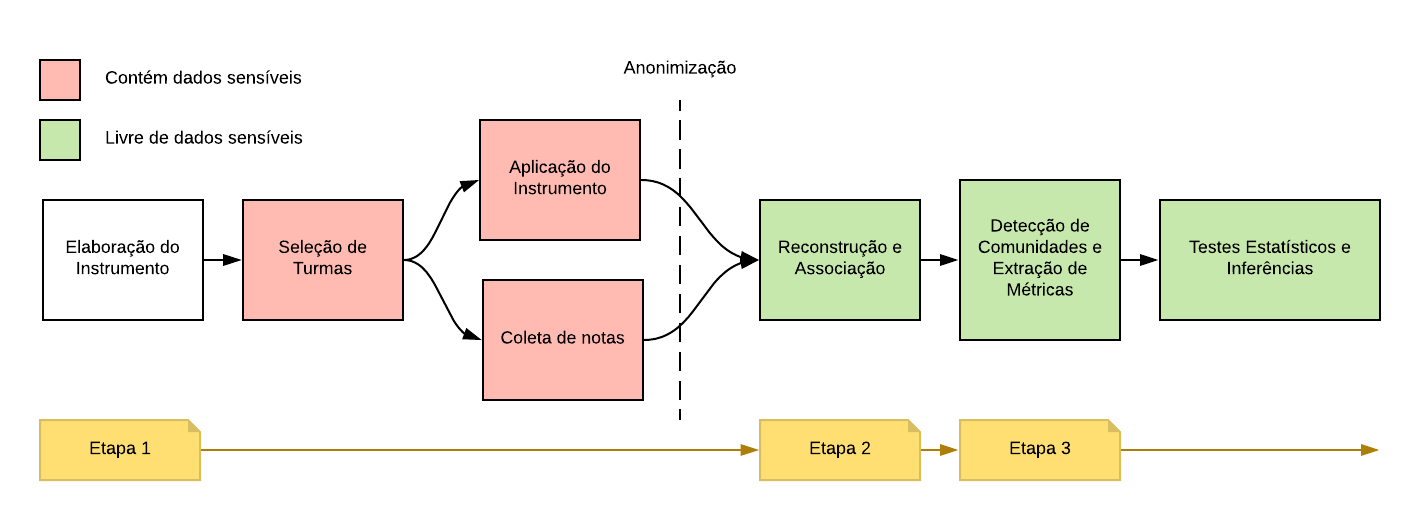
\includegraphics[width=\textwidth]{imagens/fluxo_ttc.png}
    \caption{Fluxo de atividades.}
    \label{fig:process}
    \Fonte{o autor.}
\end{figure}

\section{Coleta de Dados} \label{sec:datacollection}

A etapa de coleta de dados compreende os procedimentos que serão empregados para identificar, coletar e armazenar informações referentes aos atores das redes sociais e seus laços. Para realizá-la, será necessário consultar a população de estudantes e a instituição de ensino que os abriga, atendendo às diretrizes éticas estabelecidas. Esta etapa lidará com dados pessoais dos estudantes, que deverão ser cuidadosamente protegidos; ao seu término, tais dados serão anonimizados, eliminando vestígios pessoais dos indivíduos que os forneceram.

\subsection{Elaboração do Instrumento de Pesquisa} \label{sec:surveydesign}

Conforme identificado na Seção \ref{sec:collection}, a literatura científica estabelece que a estratégia mais comum para a coleta de dados em pesquisas na área de redes sociais é a aplicação de questionários e entrevistas, onde os próprios indivíduos sob estudo diretamente fornecem informações sobre seus laços sociais. Desta forma, assim como os três trabalhos analisados na Seção \ref{sec:relatedwork}, o presente estudo fará uso de um questionário, pois identificou-se que entrevistas consumiriam tempo demasiado devido ao número de participantes em potencial.

De forma similar ao trabalho de \citeonline{Blansky2013}, o questionário conterá uma pergunta referente ao nível de amizade com cada colega, utilizando uma escala de valores inteiros. A escala utilizada neste estudo seguirá a teoria de zonas de contato social descrita por \citeonline{Berkman2000} e apresentada na Seção \ref{sec:socialinfluence}, que estabelece seis níveis de proximidade, variando de amigos extremamente íntimos a indivíduos conhecidos apenas de rosto. Como os colegas do respondente serão identificados apenas por nome no questionário, considera-se que indivíduos que pertencem à zona mais distante, em geral, não poderão ser reconhecidos, e portanto seu valor na escala de amizade será igual a 0.

Com isso, estabe

\section{Reconstrução e Associação} \label{sec:reconstruction}
\section{Análise} \label{sec:analysiscollected}

% fluxograma das etapas

% estágio de coleta
% coleta de amizades (questionário)
% como as perguntas/opções do questionário foram feitas
% plano de coleta de dados de amizade (e-mail/turmas)
% estratégias de anonimização
% coleta de notas (comitê de ética)

% estágio de reconstrução
% formato dos dados
% missing values (distribuição normal)
% tratamento/associação de notas com alunos

% estágio de análise
% centralidade
% modularidade (D) - algoritmo do Santiago
% modelo nulo
% comunidades tem notas parecidas?
% p2 (divisão relativo/absoluto)
% p3

% testes preliminares
% figuras?
% áudios/transcrições

\section{Planejamento para o TTC II} \label{sec:plan2}

\subsection{Metodologia} \label{sec:methodology2}

IDK

\subsection{Cronograma} \label{sec:schedule}

\begin{cronograma}{Cronograma de execução para o TTC II}\label{board:schedule2}
    \uHeaderCronograma{08/2019}{09/2019}{10/2019}{11/2019}{12/2019}
    \uAtividade{3.b) Reconstrução das redes} {XXXX}{} {}{}{}
    \uAtividade{3.c) Associação dos dados}   {}    {XX \nX\nX}{}{}{}
    \uAtividade{4.a) Métricas de avaliação}  {}    {\nX\nX XX} {XXXX} {} {}
    \uAtividade{4.b) Testes estatísticos}    {}    {}         {}     {XXXX} {}
    \uAtividade{4.c) Documentação}           {}    {}         {XXXX} {XXXX} {XX \nX\nX}
\end{cronograma}

\subsection{Análise de Riscos} \label{sec:risks}

\begin{riscos}{Análise de Riscos}\label{quadro:riscos}
    \uHeaderRiscos
    \uRisco{Reprovação do projeto submetido ao Comitê de Ética}
          {Média}{Baixo}{Retorno negativo na plataforma de submissão de projetos}
          {Adaptação do projeto de acordo com as indicações dos revisores seguida de ressubmissão}
    \uRisco{Presença de dados faltantes para uma turma}
          {Alta}{Baixo}{Um ou mais membros da turma optaram por não responder o questionário}
          {Preenchimento dos dados faltantes por meio de análise de tendência média entre os membros da turma}
    \uRisco{Ausência de métricas de avaliação específicas para o problema}
          {Média}{Média}{Nenhuma das referências bibliográficas identificadas propõe uma métrica de avaliação diretamente aplicável}
          {Expansão dos termos de pesquisa em bases de artigos, seguido de adaptação ou elaboração de uma métrica específica para o problema}
\end{riscos}
